\documentclass[
  bibliography=totoc,     % Literatur im Inhaltsverzeichnis
  captions=tableheading,  % Tabellenüberschriften
  titlepage=firstiscover, % Titelseite ist Deckblatt
]{scrartcl}

% Paket float verbessern
\usepackage{scrhack}

% Warnung, falls nochmal kompiliert werden muss
\usepackage[aux]{rerunfilecheck}

% unverzichtbare Mathe-Befehle
\usepackage{amsmath}
% viele Mathe-Symbole
\usepackage{amssymb}
% Erweiterungen für amsmath
\usepackage{mathtools}

% Fonteinstellungen
\usepackage{fontspec}
% Latin Modern Fonts werden automatisch geladen
% Alternativ zum Beispiel:
%\setromanfont{Libertinus Serif}
%\setsansfont{Libertinus Sans}
%\setmonofont{Libertinus Mono}

% Wenn man andere Schriftarten gesetzt hat,
% sollte man das Seiten-Layout neu berechnen lassen
\recalctypearea{}

% deutsche Spracheinstellungen
\usepackage[english]{babel}
%BUG in Biblatex wird hiermit gefixt
\providetoggle{blx@lang@captions@english}


\usepackage[
  math-style=ISO,    % ┐
  bold-style=ISO,    % │
  sans-style=italic, % │ ISO-Standard folgen
  nabla=upright,     % │
  partial=upright,   % ┘
  warnings-off={           % ┐
    mathtools-colon,       % │ unnötige Warnungen ausschalten
    mathtools-overbracket, % │
  },                       % ┘
]{unicode-math}

% traditionelle Fonts für Mathematik
\setmathfont{Latin Modern Math}
% Alternativ zum Beispiel:
%\setmathfont{Libertinus Math}

\setmathfont{XITS Math}[range={scr, bfscr}]
\setmathfont{XITS Math}[range={cal, bfcal}, StylisticSet=1]

% Zahlen und Einheiten
\usepackage[
%  locale=DE,                   % deutsche Einstellungen
  separate-uncertainty=true,   % immer Fehler mit \pm
  per-mode=symbol-or-fraction, % / in inline math, fraction in display math
]{siunitx}

% chemische Formeln
\usepackage[
  version=4,
  math-greek=default, % ┐ mit unicode-math zusammenarbeiten
  text-greek=default, % ┘
]{mhchem}

% richtige Anführungszeichen
\usepackage[autostyle]{csquotes}

% schöne Brüche im Text
\usepackage{xfrac}

% Standardplatzierung für Floats einstellen
\usepackage{float}
\floatplacement{figure}{htbp}
\floatplacement{table}{htbp}

% Floats innerhalb einer Section halten
\usepackage[
  section, % Floats innerhalb der Section halten
  below,   % unterhalb der Section aber auf der selben Seite ist ok
]{placeins}

% Seite drehen für breite Tabellen: landscape Umgebung
\usepackage{pdflscape}

% Captions schöner machen.
\usepackage[
  labelfont=bf,        % Tabelle x: Abbildung y: ist jetzt fett
  font=small,          % Schrift etwas kleiner als Dokument
  width=0.9\textwidth, % maximale Breite einer Caption schmaler
]{caption}
% subfigure, subtable, subref
\usepackage{subcaption}

% Grafiken können eingebunden werden
\usepackage{graphicx}

% Grafiken rotieren
\usepackage{rotating}

% Grafiken zentriert überstehen lassen
\usepackage{adjustbox}

% größere Variation von Dateinamen möglich
\usepackage{grffile}

% schöne Tabellen
\usepackage{booktabs}

% Verbesserungen am Schriftbild
\usepackage{microtype}

% Literaturverzeichnis
\usepackage[
  backend=biber,
]{biblatex}
% Quellendatenbank
\addbibresource{lit.bib}
\addbibresource{programme.bib}

% Hyperlinks im Dokument
\usepackage[
  german,
  unicode,        % Unicode in PDF-Attributen erlauben
  pdfusetitle,    % Titel, Autoren und Datum als PDF-Attribute
  pdfcreator={},  % ┐ PDF-Attribute säubern
  pdfproducer={}, % ┘
]{hyperref}
% erweiterte Bookmarks im PDF
\usepackage{bookmark}

% Trennung von Wörtern mit Strichen
\usepackage[shortcuts]{extdash}

%Bra und Ket 
\newcommand\bra[2][]{#1\langle {#2} #1\rvert}
\newcommand\ket[2][]{#1\lvert {#2} #1\rangle}

\author{%
  Christopher Breitfeld\\%
  \href{mailto:christopher.breitfeld@tu-dortmund.de}{christopher.breitfeld@tu-dortmund.de}%
  \and%
  Henry Krämerkämper\\%
  \href{mailto:henry.kraemerkaemper@tu-dortmund.de}{henry.kraemerkaemper@tu-dortmund.de}%
}
\publishers{TU Dortmund – Fakultät Physik}



\subject{V46}
\title{Faraday-Effekt an Halbleitern}
\date{%
  Durchführung: 2. Mai 2022
  \hspace{3em}
  Abgabe: \today
}

\begin{document}

\maketitle
\thispagestyle{empty}
\tableofcontents
\newpage

%\section{Vorbereitung}
\label{sec:vorbereitung}
\subsection{Energiestruktur des Atoms}

\subsubsection{Welche Quantenzahlen definieren den Zuestand des Elektrons im Wasserstoffatom?}
$\ket{n,l,m}$
\begin{itemize}
    \item n: Haupt-QZ
    \item l: Bahndrehimpuls QZ
    \item m: magnetische QZ
\end{itemize}

\subsubsection{Was ist die Feinstruktur (Spin-Bahn-Kopplung)?}
\begin{itemize}
    \item WW zwischen Bahndrehimpuls $L$ und Spin $S$
    \item Halbklassisch: 
        \to im Bezugssys. des Elektrons stellt der Kern einen Kreistrom um das Elektron dar
        \to Kreisströme verursachen magnetisches Feld (Biot-Savart) (Kreisstrom entspricht dem Bahndrehimpuls)
        \to dieses magnetische Feld wechselwirkt mit dem magnetischen Moment des Elektronen-Spins
        \to klassisches Analogon: Stabmagnet in Spule
    \item in nicht-relativistischer QM wird ein Störterm $H_S\propto\vec{L}\cdot\vec{S}$ ergänzt
    \item in relativistischer QM ergibt sich die WW automatisch aus der Dirac-Gleichung
\end{itemize}

\subsubsection{Beschreiben Sie die Elektronenkonfiguration und Drehimpulskopplungen in Mehrelektronenatomen (LS-Kopplung und jj-Kopplung)}
\begin{itemize}
    \to Stärke der Spin-Bahn-WW nimmt mit steigendem $Z$ stark zu
    \to Stärke der Spin-Bahn-WW nimmt mit steigendem $n$ ab
\end{itemize}
jj-Kopplung:
\begin{itemize}
    \item Gesamtdrehimpuls aller einzelnen Teilchen werden addiert
    \begin{equation*}
        J=\sum_i j_i=\sum_i(l_i+s_i)\\
    \end{equation*}
    \item elektrostatische Störung der Elektronen untereinander vernachlässigt
    \to Spin-Bahn-WW jedes einzelnen Elektrons >> elektrostatische Störung der Elektronen untereinander
    \iff gute Näherung für mittelschwere Atome auf inneren Schalen & schwere Atome auf ganzen Hülle
\end{itemize}
LS-Kopplung: 
\begin{itemize}
    \item Bahndrehimpuls aller Teilchen und Spin aller Teilchen werden addiert
        \begin{equation*}
            J=L+S=\sum_il_i + \sum_i s_i
        \end{equation*}
    \item Spin-Bahn-WW wird vernachlässigt \iff L & S sind gute QZ 
    \to elektrostatische Störung der Elektronen untereinander >> Spin-Bahn-WW jedes einzelnen Elektrons
    \to gute Näherung für leichte Atome
\end{itemize}


\subsection{Magnetisches Moment des Atoms}

\subsubsection{Wie ist der Zusammenhang zwischen dem magnetischen Moment eines Elektrons und seinen Drehimpulsquantenzahlen?}
\begin{align*}
    \vec{\mu_L}&=-\frac{g_L\mu_B}{\hbar}\vec{L}=-g_L\mu_B\sqrt{l(l+1)}, \quad g_L\approx 1\\
    \vec{\mu_S}&=-\frac{g_S\mu_B}{\hbar}\vec{S}=-g_S\mu_B\sqrt{s(s+1)}, \quad g_S\approx 2
\end{align*}
\subsubsection{Was ist der Unterschied zwischen dem gyromagnetischen Verhältnis für den Elektronenspin und demjenigen für den Drehimpuls?}
\begin{align*}
    \gamma=\frac{|\vec{\mu_l}|}{|\vec{l}|} \qquad
    \gamma=\frac{|\vec{\mu_s}|}{|\vec{s}|}
\end{align*}

\subsection{Aufspaltung des Energieniveaus eines Atoms im homogenen Magnetfeld}

\subsubsection{In wie viele Niveas spaltet sich der Zustand mit Gesamtdrehimpuls J?}
\subsubsection{Wie ändert sich die Aufspaltung mit der Magnetfeldstärke?}
\subsubsection{Was versteht man unter dem Paschen-Back-Effekt?}
\subsection{Optische Übergänge zwischen Zeemannaufgespaltenen Energieniveaus}
\subsubsection{Zwischen welchen Zuständen sind optische Übergänge erlaubt?}
\subsubsection{Wie viele Spektrallinien beobachtet man im normalen und anormalen Zeeman-Effekt?}
\subsubsection{Wie sind die Spektrallinien polarisiert?}
\textit{Beachten Sie die geomatrischen Verhältnisse des Experiments, d.h. wie ändert sich das Spektrum und die Polarisation der Linien
bei der Beobachtung entlang der Magnetfeldrichtung (longitudinale Geometrie) oder senkrecht zur Magnetfeldrichtung (transversale
Geometrie)?}
\subsection{Optische Übergänge in Cd Atomen}
\subsubsection[]{Stellen Sie das Termschema für die rote $(^1P_1 \leftrightarrow ^1D_2)$ und blaue 
$(^3S_1 \leftrightarrow ^3P_1)$ Linie der Cd-Lampe auf.}
\subsubsection[]{Berechnen Sie die Landé-Faktoren $g_i$ und die Aufspaltung $\Delta E$ der Zeeman-Linie.}
\subsubsection{Zeichnen Sie die erwartetden Spektren.}
\subsubsection{Wie viele Linien erwarten Sie im Magnetfeld?}
\subsubsection{Ordnen Sie den beobachtbaren Linien ihre Polarisation zu.}
\subsection{Dispersionsgebiet und spektrale Auflösung der Messapparatur}
\subsubsection[]{Berechnen Sie für $\lambda=\SI{643.8}{\nano\metre}$ und $\lambda=\SI{480}{\nano\metre}$ das Dispersionsgebiet 
$\Delta\lambda_D$  und das Auflösevermögen $A$ der Lummer-Gehrcke-Platte ($d=\SI{4}{\milli\metre}, L=\SI{120}{\milli\metre}, 
n(\SI{643.8}{\nano\metre})=\num{1.4567}, n(\SI{480}{\nano\metre})=\num{1.4635}$).}
\subsection{Optimale Einstellung der Magnetfeldstärke}
\subsubsection[]{Bestimmen Sie die Bedingung für die optimale Aufspaltung $\Delta\lambda$.}
\textit{Die Messung ist nur sinnvoll für die Aufspaltung innerhalb des Dispersionsgebiets $\Delta\lambda_D$. Das bedeutet, dass 
es eine Begrenzung für die Magnetfeldstärke gibt.}
\subsubsection{Dauras schätzen Sie die entsprechende optimale Magnetfeldstärke für jede spektrale Linie, die Sie anschließend
messen sollen.}
\section{Einleitung}
\label{sec:einleitung}

\section{Theoretischer Hintergrund des Versuches}
\label{sec:Theorie}
\subsection{Eigenschaften des Myons}
\label{subsec:Eigenschaften}
Myonen sind Leptonen aus der zweiten der drei Leptonenfamilien. Sie haben
eine Ruhemasse von $\SI{105.66}{\mega\electronvolt}$ sowie eine Lebensdauer
von $\SI{2.197}{\micro\second}$. Das Myon $\mu^{-}$ ist einfach negativ geladen,
das Antimyon $\mu^{+}$ daher einfach positiv.\cite{PDG}
Myonen unterliegen wie alle Fermionen der schwachen und der elektromagnetischen
Wechselwirkung.
\subsection{Entstehung von kosmischer Strahlung}
\label{subsec:kosmischeStrahlung}
Als primäre kosmische Strahlung werden hochenergetische Teilchen bezeichnet, welche
in der Sonne und anderen Sternen entstanden sind. Sie besteht hauptsächlich aus Protonen.
Diese wechselwirken mit Teilchen in der Atmosphäre, was elektromagnetische
Schauer erzeugt. In diesen Schauern entstehen Sekundärteilchen. Bei diesen
Sekundärteilchen handelt es sich hauptsächlich um Pionen und Kaonen.
\begin{figure}
  \centering
  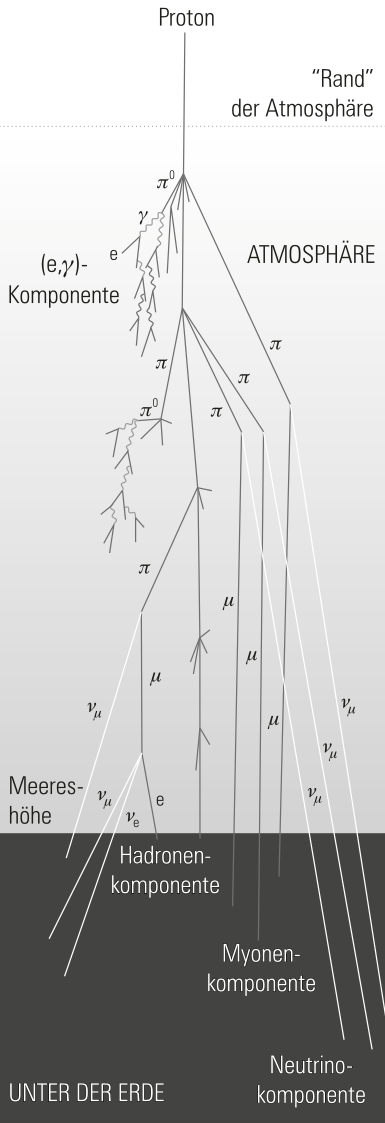
\includegraphics[width=0.2\textwidth]{pictures/Schauer.png}
  \caption{Schematische Darstellung eines EM-Schauers kosmischer Strahlung. \cite{Q1}}
  \label{fig:schauer}
\end{figure}
\noindent
Die so entstandenen Pionen zerfallen aufgrund der Helizitätsunterdrückung
des Zerfalls
\begin{align*}
  \pi^{-} & \rightarrow e^{-} + \bar{\nu}_{e} \\
  \pi^{+} & \rightarrow e^{+} + \nu_{e}
\end{align*}
\noindent
hauptsächlich über die Zerfallskanäle
\begin{align*}
\pi^{-} & \rightarrow \mu^{-} + \bar{\nu}_{\mu} \\
\pi^{+} & \rightarrow \mu^{+} + \nu_{\mu}.
\end{align*}
\noindent
Der Zerfall der Kaonen verhält sich analog. Die aus kosmischer Strahlung entstandenen
Myonen werden kosmische Myonen genannt.
Sie zerfallen, wie in Abbildung \ref{zerfall} dargestellt, über die schwache Wechselwirkung.
\begin{figure}[H]
  \centering
  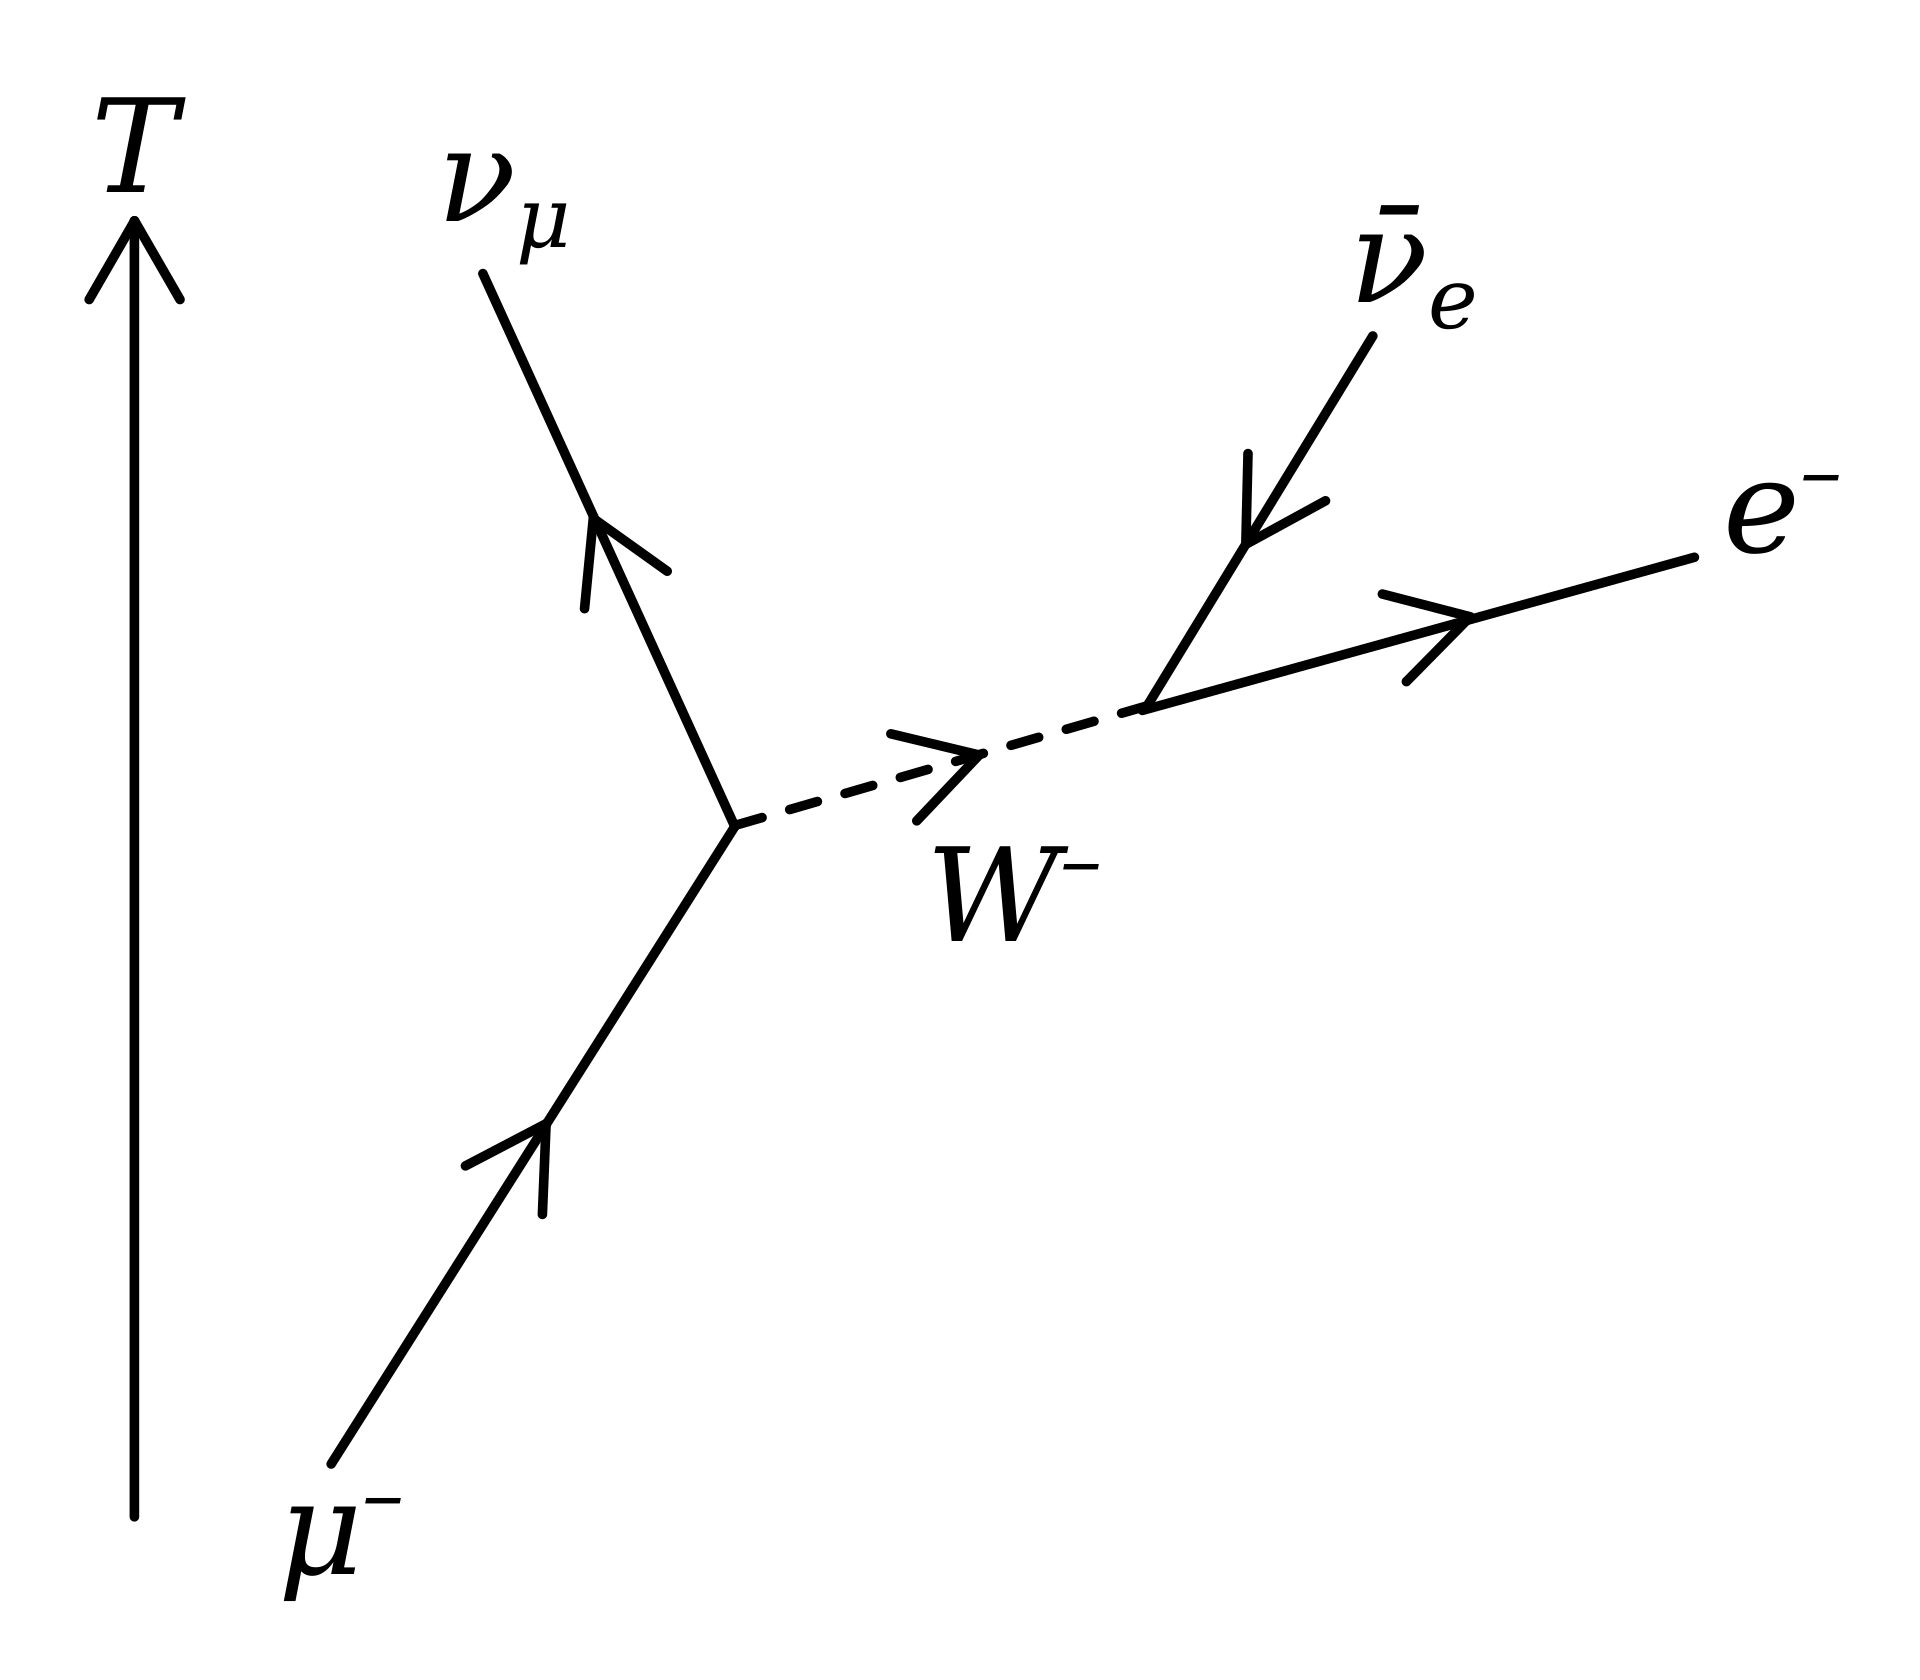
\includegraphics[width=0.5\textwidth]{pictures/Muon_Decay.png}
  \caption{Feynman-Graph des Myonenzerfalls.\cite{Myon-Wikipedia}}
  \label{zerfall}
\end{figure}
\noindent
Teilchenzerfälle sind statistische Prozesse. Daher wird dem Zerfall des Myons
eine Wahrscheinlichkeit $\text{d}W$  zugeordnet, mit der dieser in einer bestimmten Zeit $\text{d}t$
stattfindet:
\begin{equation*}
  \text{d}W = \lambda \text{d}t.
\end{equation*}
\noindent
Hierbei ist der Proportionalitätsfaktor $\lambda$ die Zerfallskonstante.
Die Zerfallskonstante und die mittlere Lebensdauer eines Teilchens haben den folgenden
Zusammenhang:
\begin{equation*}
  \lambda = \frac{1}{\tau}.
\end{equation*}
\noindent
Die mittlere Lebensdauer beschreibt die Zeit, nach der sich die Anzahl der Teilchen um
den Faktor $e \approx 2.7$ verringert hat.
Für die Änderung der Teilchenzahl $N$ in einem Zeitraum $\text{d}t$ gilt
\begin{equation}
  \text{d}N = - N \cdot \text{d}W = - N \cdot \lambda \text{d}t.
  \label{eqn:zerfall1}
\end{equation}
\noindent
Durch Integration der Gleichung \ref{eqn:zerfall1} kann das Zerfallsgesetz hergeleitet werden:
\begin{equation}
  N(t) = N_{0} \cdot \exp{(-\lambda t)}.
  \label{eqn:zerfallsgesetz}
\end{equation}
\noindent
\subsection{Bestimmung der mittleren Lebensdauer der Myonen}
\label{subsec:BestimmungLebensdauer}
Um die kosmischen Myonen zu detektieren, wird ein organischer Szintillator verwendet.
Szintillatoren erzeugen bei Eintritt eines geladenen Teilchens einen Lichtpuls.
Dieser entsteht, da durch Eintritt eines geladenen Teilchens Moleküle des Szintillators
angeregt werden, welche dann unter Abgabe von Photonen wieder in ihre Grundzustände zurückfallen.
Diese Lichtpulse können in elektrische Signale umgewandelt und weiterverarbeitet werden.
Bei Eintritt eines Myons in den Szintillator wird ein Signal gemessen. Wenn das Myon innerhalb
des Szintillators, wie in der Abbildung \ref{zerfall} dargestellt, zerfällt, kann auch von den Zerfallsprodukten
ein Signal detektiert werden. Dies ist der Fall, wenn das Myon seine gesamte kinetische Energie
an das Szintillatormaterial abgibt.
Durch Messung der Zeit zwischen dem Eintritt des Myons und des
Zerfalls ist eine Bestimmung der mittleren Lebensdauer des Myons möglich. Es wird also
innerhalb eines bestimmten Zeitrahmens nach Eintritt eines Myons auf ein weiteres Signal
gewartet. Wenn innerhalb dieses Zeitrahmens ein weiteres Myon den Detektor erreicht oder wenn
ein Myon nicht innerhalb des Detektors zerfällt, kann die Messung verfälscht werden, da
Zerfälle, welche außerhalb des Messzeitrahmens stattfinden, nicht gemessen werden.
Diese Verfälschungen der Messung erzeugen einen Untergrund. Dieser lässt sich mithilfe
einer Poissonverteilung abschätzen. Dies ist in folgender Gleichung angegeben:
\begin{equation}
  U = P_{\lambda} (k) = \frac{\lambda^{k}}{k!} \exp{(-\lambda)},
  \label{eqn:Untergrundrate}
\end{equation}
\noindent
mit dem Erwartungswert der Poissonverteilung $\lambda$ und der Ereignisanzahl $k$.

\section{Durchführung des Versuches}
\label{sec:Durchführung}
\subsection{Aufbau des Versuches}
\label{subsec:Aufbau}
Organische Szintillatoren haben gegenüber anorganischen Szintillatoren den Vorteil, dass sie eine sehr
gute Zeitauflösung besitzen. Da eine gute Zeitauflösung instrumental für die Qualität der genommenen
Daten ist, wird in diesem Versuch ein organischer Szintillator verwendet.
Dieser Szintillator befindet sich in einem Detektortank mit einem Volumen $V = \SI{50}{\liter}$.
Der Lichtpuls des Szintillators wird durch einen Photovervielfacher (im englischen Sprachraum: Photomultipliertube,
daher oft abgekürzt als PMT) in ein elektrisches Signal umgewandelt und verstärkt.
Dabei können durch thermische Effekte Elektronen emittiert werden, welche die
Messung verfälschen würden. Daher werden zwei PMTs verwendet, welche durch eine
Koinzidenzschaltung miteinander verbunden sind. So werden nur Signale verwendet, welche
von beiden PMTs nachezu gleichzeitig ausgesandt werden, was Fehler durch thermische
Effekte vermeidet.
Die Schaltung ist in folgender Abbildung dargestellt.
\begin{figure}[H]
  \centering
    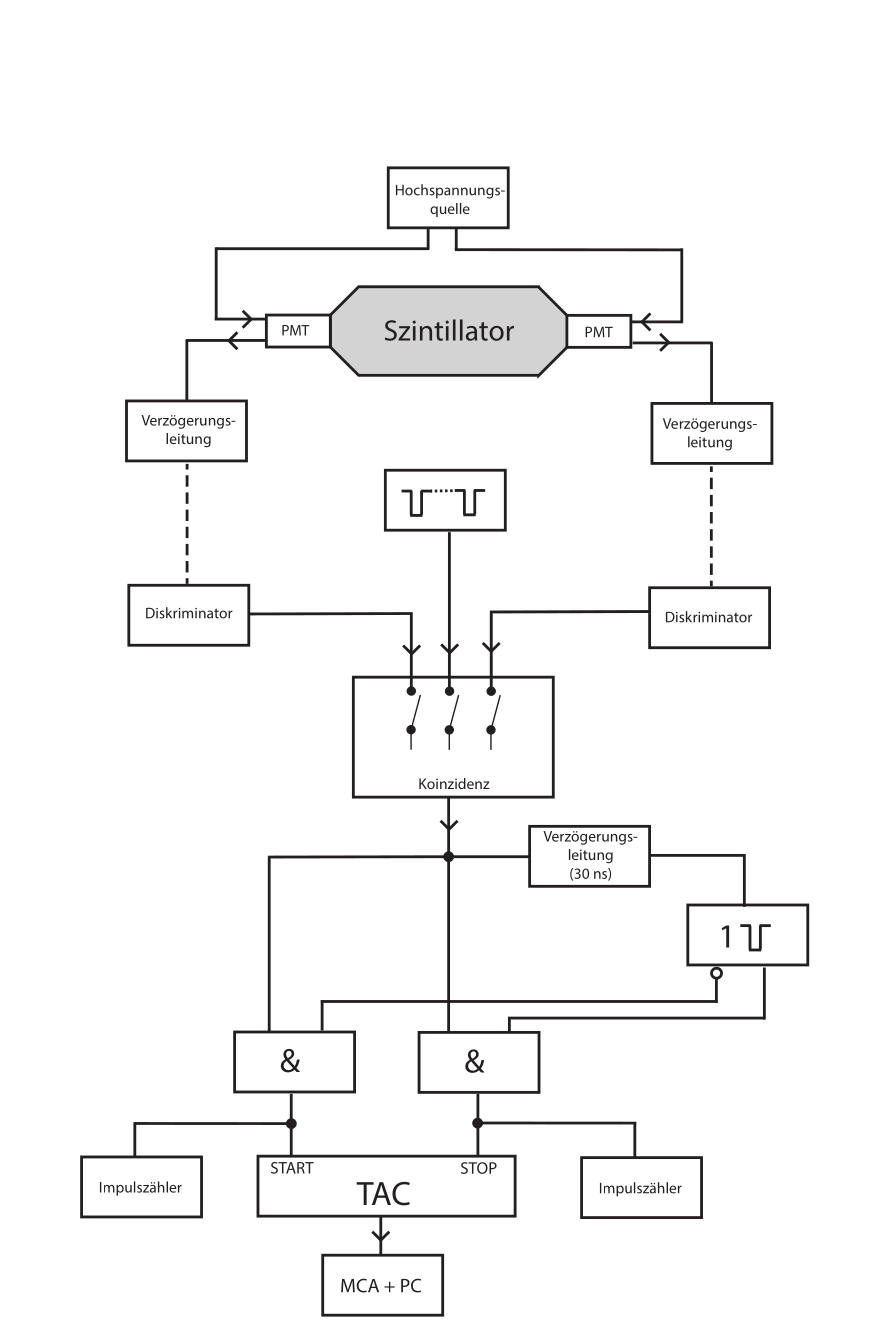
\includegraphics[width=0.7\textwidth]{pictures/Schaltbild.png}
    \caption{Schaltbild des Versuchsaufbaus. \cite{versuchsbeschreibung}}
    \label{fig:Schaltbild}
\end{figure}
\noindent
Das Signal der PMTs wird über eine Verzögerungsleitung, welche schaltungstechnische Unterschiede
wie z.B. Kabelwege ausgleicht, durch einen Diskriminator geleitet. Dieser lässt nur Signale ab
einer gewissen Schwelle hindurch. Diese Schwelle lässt sich einstellen, wodurch Rauschen
minimiert werden kann. Das elektrische Signal, welches von dem Diskriminator ausgegeben wird,
kann auf verschiedene Breiten eingestelt werden. Hiernach folgt die bereits erwähnte Koinzidenz.
Die nun folgende Schaltung funktioniert wie eine Stoppuhr, welche das Warten auf ein Zerfallssignal
nach einer Suchzeit $T_{\text{S}}$ abbricht, was nötig wird, wenn das Myon nicht innerhalb des Detektors
zerfällt. Dies ist realisiert mittels zweier AND-Gatter, welche beide das Signal erhalten. Zusätzlich
wird das Signal auch über eine Verzögerungsleitung in einen Monoflop gesendet, welcher einen negierten
Ausgang zum linken AND-Gatter und einen normalen Ausgang zum rechten AND-Gatter besitzt. Erhält der
Monoflop das erste Signal, wird über den negierten Ausgang in das linke AND-Gatter ein Start-Signal zum
Time-to-Amplitude Converter (TAC) gesendet. Dies startet die Suchzeit. Nach Ablauf selbiger oder
nach Erhalt eines weiteren Signals sendet der Monoflop ein Signal über den normalen Ausgang in
das rechte AND-Gatter, welches ein Stop-Signal an den TAC sendet.
Der TAC wandelt die Zeitspanne zwischen Start-Signal und Stop-Signal in eine Amplitude, dessen Höhe der
Länge der Zeitspanne entspricht, um.
Der TAC ist verbunden mit einem Vielkanalanalysator (im englischen Sprachraum Multi-Channel Analyser, daher abgekürzt als MCA).
Der MCA sortiert die erhaltenen Amplituden nach ihrer Höhe in ein Histogramm, welches von einem
angeschlossenen Computer ausgelesen und gespeichert werden kann.
Zusätzlich sind an Start- und Stop-Eingang des MCAs Impulszähler verbunden, sodass für eine Abschätzung
des Untergrundes auch die Myonen gezählt werden, welche nicht im Detektor zerfallen.
\subsection{Justage des Versuchsaufbaus}
\label{JustageVersuchsaufbau}
Bevor die Messung durchgeführt werden kann, muss die nach Abbildung~\ref{fig:Schaltbild} aufgebaute Schaltung justiert
werden. Die Diskriminatoren werden so eingestellt, das in etwa $30$ Impulse pro Sekunde gemessen werden können.
Die Breite eines Pulses der Diskriminatoren wird einmal auf $\Delta t_\text{Puls} = \SI{15}{\nano\second}$ und einmal auf $\Delta t_\text{Puls} = \SI{10}{\nano\second}$
eingestellt, womit später auch die eigentliche Messung durchgeführt wird. Die Verzögerungsleitungen werden separat
variiert, um die Ereignisrate zu maximieren. Die Suchzeit des Monoflops muss auf $T_{\text{S}} = \SI{10}{\micro\second} $ eingestellt werden.
Unter Verwendung des Doppelimpulsgenerators wird der TAC kalibriert. Es werden verschiedene Impulsabstände eingestellt
und diese dann den einzelnen Kanälen zugeordnet. Dies wird mit mindestens $10$ Werten zwischen $\SI{0.3}{\micro\second}$
und $\SI{9.9}{\micro\second}$ durchgeführt.

\section{Auswertung der Messdaten}
\label{sec:Auswertung}

\subsection{Eichung des Magnetfeldes}
\label{sec:magnetfeld}
Die bei der Messung des Magnetfeldes aufgenommenen Daten sind in Tabelle \ref{tab:B} aufgelistet.

\begin{table}[H]
    \centering
      \caption{Magnetfeldstärke $B$ für verschiedene Stromstärken $I$.}
      \label{tab:B}
      \sisetup{table-format=3.1}
      \begin{tabular}{S[table-format=1.1] S}
        \toprule
        {$I[\si{\ampere}]$} & {$B[\si{\milli\tesla}]$}\\
        \midrule
        0   &   7.3    \\       
        1   &   106.2  \\
        2   &   206.2  \\
        3   &   301.9  \\
        4   &   388.4  \\
        5   &   462.8  \\
        6   &   522.9  \\
        7   &   560.2  \\
        7.5 &   577.5  \\
        \bottomrule
      \end{tabular}
\end{table}
\noindent

Für diese Messwerte wurde mittels \textit{numpy.polyfit} \cite{numpy} eine Regression der Form 
\begin{equation}
  B=aI^3+bI^2+cI+d \label{eqn:B}
\end{equation}
durchgeführt. Diese ist in Abbildung \ref{fig:B} visualisiert. 

\begin{figure}[H]
    \centering
    \includegraphics[scale= 0.8]{build/magnet.pdf}
    \caption{Magnetfeldstärke $B$ für verschiedene Stromstärken $I$ mit Regression.}
    \label{fig:B}
\end{figure}
\noindent

Die berechneten Parameter der Regression \ref{eqn:B} ergeben sich zu
\begin{align*}
    a&=\SI{-0.59\pm 0.06}{\milli\tesla\per\cubic\ampere}\\
    b&=\SI{1.20 \pm 0.66}{\milli\tesla\per\square\ampere}\\
    c&=\SI{99.91\pm 2.05}{\milli\tesla\per\ampere}\\
    d&=\SI{6.68 \pm 1.64}{\milli\tesla} .
\end{align*}

\subsection{Auswertung der roten Spektrallinie}
\label{sec:rot}
Für die rote Spektrallinie wurden während der Messung die Bilder \ref{fig:rot} und \ref{fig:rot_sigma} 
aufgenommenen. Dabei ist in Abbildung \ref{fig:rot} das Interferenzmuster ohne Magnetfeld und in 
Abbildung \ref{fig:rot_sigma} das Interferenzmuster mit Magnetfeld abegebildet. Der Elektromagnet wurde 
bei einer Stromstärke von $I=\SI{7.5}{\ampere}$ betrieben, was nach Kapitel \ref{sec:magnetfeld} einem 
Feld von $B=\SI{577.5}{\milli\tesla}$ entspricht.

\begin{figure}[H]
    \centering
    
\includegraphics[scale= 0.2]{Messung/Rot[6].JPG}
    \caption{Interferenzmuster der roten Spektrallinie ohne Magnetfeld.}
    \label{fig:rot}
\end{figure}
\noindent

\begin{figure}[H]
    \centering
    
\includegraphics[scale= 0.2]{Messung/Rot_Sigma[7].JPG}
    \caption{Interferenzmuster der roten Spektrallinie beim $\sigma$-Übergang.}
    \label{fig:rot_sigma}
\end{figure}
\noindent
Zur Bestimmung des Lande-Faktors wurden mittels \textit{Affinity Designer} \cite{affinity} die Abstände $\Delta s$ 
in Abbildung \ref{fig:rot} und $\delta s$ in Abbildung \ref{fig:rot_sigma} bestimmt. Die Abstände sind in 
Tabelle \ref{tab:rot} enumeriert.

\begin{table}[H]
    \centering
      \caption{Messwerte für die Linienabstände $\Delta s$ und die Aufspaltung $\delta s$ in Pixeln für die rote Spektrallinie.}
      \label{tab:rot}
      \sisetup{table-format=2.1}
      \begin{tabular}{S[table-format=3.1] S}
        \toprule
        {$\Delta s[\text{px}]$} & {$\delta s[\text{px}]$}\\
        \midrule
        117.9  &  59.2 \\
        128.2  &  56.0 \\
        134.4  &  53.3 \\
        144.6  &  55.1 \\
        149.8  &  63.3 \\
        160.6  &  72.0 \\
        178.7  &  74.7 \\
        202.4  &  84.9 \\
        \bottomrule
      \end{tabular}
\end{table}
\noindent
Die mit \textit{NumPy} \cite{numpy} bestimmten Mittelwerte mit Standardabweichung lauten
\begin{align*}
    \overline{\Delta s}&=\num{152.1\pm 26.0}\text{px}\\
    \overline{\delta s}&=\num{64.81\pm 64.8}\text{px} .
\end{align*}
Einsetzen in Gleichung \ref{eqn:gebiet} ergibt für Dispersionsgebiet
\begin{equation*}
  \delta\lambda=\SI{10.4\pm 2.5}{\pico\metre} .
\end{equation*}
Der Landefaktor $g$ berechnet sich nach Gleichung \ref{eqn:aufspaltung} zu 
\begin{equation*}
  g=\num{0.93\pm0.22} .
\end{equation*}

\subsection{Auswertung der blauen Spektrallinie}
\label{sec:blau}
Für die Untersuchung des anormalen Zeeman-Effekts werden zwei verschiedene Magnetfeldstärken verwendet, um 
die $\pi$- von den $\sigma$-Übergängen unterscheiden zu können. Die Bestimmung von $\Delta s$ wird für beide 
Übergänge an Abbildung \ref{fig:blau} vorgenommen. 

\begin{figure}[H]
    \centering
    
\includegraphics[scale= 0.2]{Messung/Blau[3].JPG}
    \caption{Interferenzmuster der blauen Spektrallinie ohne Magnetfeld.}
    \label{fig:blau}
\end{figure}
\noindent

\subsubsection[]{$\sigma$-Übergang}
\label{sec:sigma}

In Abbildung ist Interferenzmuster der blauen Spektrallinie für eine Stromstärke von $I=\SI{4.5}{\ampere}$
dargestellt. Dieser Stromstärke entspricht nach der Regression \ref{eqn:B} eine Feldstärke von 
$B=\SI{426.7}{\milli\tesla}$. 
\begin{figure}[H]
    \centering
    
\includegraphics[scale= 0.2]{Messung/Blau_Sigma[4].JPG}
    \caption{Interferenzmuster der blauen Spektrallinie beim $\sigma$-Übergang.}
    \label{fig:blau_sigma}
\end{figure}
\noindent
Die mit \textit{Affinity Designer} \cite{affinity} bestimmten Abstände $\Delta s$ und $\delta s$ sind in Tabelle \ref{tab:blau_sigma}
angeführt.

\begin{table}[H]
    \centering
      \caption{Messwerte für die Linienabstände $\Delta s$ und die Aufspaltung $\delta s$ in Pixeln für den $\sigma$-Übergang der blaue Spektrallinie.}
      \label{tab:blau_sigma}
      \sisetup{table-format=2.1}
      \begin{tabular}{S[table-format=3.1] S}
        \toprule
        {$\Delta s[\text{px}]$} & {$\delta s[\text{px}]$}\\
        \midrule
        84.4  &  60.7  \\
        92.0  &  65.7  \\
        96.8  &  64.1  \\
        99.0  &  70.6  \\
        104.4 &  75.0  \\
        108.0 &  76.5  \\
        114.0 &  86.2  \\
        118.0 &  89.8  \\
        131.0 &  104.9 \\
        140.7 &  106.7 \\
        147.1 &  113.7 \\
        166.0 &  139.7 \\
        190.6 &  128.3 \\
        \bottomrule
      \end{tabular}
\end{table}
\noindent
Doe Mittelwerte werden mit \textit{NumPy} \cite{numpy} als 
\begin{align*}
    \overline{\Delta s}&=\num{122.5\pm 30.1}\text{px}\\
    \overline{\delta s}&=\num{90.92\pm 45.5}\text{px}
\end{align*}
ermittelt. Daraus ergibt sich mit Gleichung \ref{eqn:gebiet} zu 
\begin{equation*}
  \delta\lambda=\SI{10.0 \pm 3.7}{\pico\metre},
\end{equation*}
sodass sich der Landefaktor mit Gleichung \ref{eqn:aufspaltung} zu
\begin{equation*}
  g=\num{2.18 \pm 0.80}
\end{equation*}
bestimmen lässt.

\subsubsection[]{$\pi$-Übergang}
\label{sec:pi}
Das Interferenzmuster \ref{fig:blau_pi} wurde bei einer Stromstärke von $I=\SI{7.5}{\ampere}$ aufgenommenen. 
Der Elektromagnet hat demnach ein Magnetfeld von $B=\SI{577.5}{\milli\tesla}$ erzeugt. 
\begin{figure}[H]
    \centering
    
\includegraphics[scale= 0.2]{Messung/Blau_Pi[5].JPG}
    \caption{Interferenzmuster der blauen Spektrallinie beim $\pi$-Übergang.}
    \label{fig:blau_pi}
\end{figure}
\noindent
Die in Tabelle \ref{tab:blau_pi} gelisteten Werte von $\Delta s$ und $\delta s$ wurden erneut mit \textit{Affinity Designer} \cite{affinity}
bestimmt.

\begin{table}[H]
    \centering
      \caption{Messwerte für die Linienabstände $\Delta s$ und die Aufspaltung $\delta s$ in Pixeln für den $\pi$-Übergang der blaue Spektrallinie.}
      \label{tab:blau_pi}
      \sisetup{table-format=2.1}
      \begin{tabular}{S[table-format=3.1] S}
        \toprule
        {$\Delta s[\text{px}]$} & {$\delta s[\text{px}]$}\\
        \midrule
        84.4  &  30.0 \\
        92.0  &  33.5 \\
        96.8  &  37.0 \\
        99.0  &  38.2 \\
        104.4 &  40.5 \\
        108.0 &  41.8 \\
        114.0 &  44.5 \\
        118.0 &  41.5 \\
        131.0 &  44.4 \\
        140.7 &  47.9 \\
        147.1 &  53.3 \\
        166.0 &  53.2 \\
        190.6 &  55.1 \\
        \bottomrule
      \end{tabular}
\end{table}
\noindent
Die Mittelwerte der Messwerte sind 
\begin{align*}
    \overline{\Delta s}&=\num{122.5\pm 30.1}\text{px}\\
    \overline{\delta s}&=\num{33.6 \pm 10.5}\text{px},
\end{align*}
woraus sich ein Dispersionsgebiet von 
\begin{equation*}
  \delta\lambda=\SI{3.70\pm 1.47}{\pico\metre}
\end{equation*}
ergibt. Dies führt schlussendlich nach Gleichung \ref{eqn:aufspaltung} zu einem Landefaktor von 
\begin{equation*}
  g=\num{0.60\pm 0.24} .
\end{equation*}

\section{Diskussion der Ergebnisse}
\label{sec:Diskussion}
Für die Diskussion der Messung wird die prozentuale Abweichung $p$ der in Kapitel \ref{sec:Auswertung} bestimmten Landefaktoren $g$ 
zu dem Theoriewerten mittels
\begin{equation*}
    p=\frac{|g_\text{theo}-g_\text{exp}|}{g_\text{theo}}
\end{equation*}
berechnet. Eine Auflistung der Werte ist in Tabelle \ref{tab:p} gegeben.

\begin{table}[H]
    \centering
      \caption{Experimentell bestimme Landefaktoren $g_\text{exp}$, Theoriewerte $g_\text{theo}$ und prozentuale Abweichung $p$.}
      \label{tab:p}
      \sisetup{table-format=1.2}
      \begin{tabular}{c S S @{${}\pm{}$} S S[table-format=2.0]  @{${}\pm{}$} S[table-format=2.0] }
        \toprule
        {Spektrallinie} & {$g_\text{theo}$} & \multicolumn{2}{c}{$g_\text{exp}$} & \multicolumn{2}{c}{$p [\%]$}\\
        \midrule
        $\text{rot},\sigma$  & 1    &  0.93 & 0.22 & 7  & 22 \\
        $\text{blau},\sigma$ & 1.75 &  1.03 & 0.31 & 41 & 18 \\
        $\text{blau},\pi$    & 0.5  &  0.60 & 0.24 & 19 & 47 \\
        \bottomrule
      \end{tabular}
\end{table}
\noindent
Insbesondere stimmen die berechneten Werte für die blaue $\pi$-Linie und die rote $\sigma$-Linie im Rahmen der 
Unsicherheit mit den Theoriewerten überein. 

\noindent
Mögliche Gründe für die Abweichungen liegen vor allem in technischen Problemen des Elektromagneten und der 
Abschätzung der Abstände $\Delta s$ und $\delta s$.
Der Elektromagnet erwärmt sich bei längerer Inbetriebnahme, was dazu führen kann, dass das Magnetfeld
teilweise oder komplett abgeschaltet wird. Die Erwärmung kann dazu führen, dass die Feldstärke während 
der Messung nicht mehr mit der in Kapitel \ref{sec:magnetfeld} geeichten Feldstärke übereinstimmt. 
%Zudem können auch inhomogene Anteile des Magnetfeldes die Messung negativ beeinträchtigt haben. 
Für die optimale Auflösung der blauen $\pi$-Linie wird nach~\ref{tab:magnet} ein Magnetfeld
von $B=\SI{1.25}{T}$ benötigt. Diese Feldstärke war mit dem vorhandenen Elektromagneten nicht zu erreichen.
Die Auflösung des Bildes \ref{fig:blau_pi} und somit auch die Abschätzung von $\delta s$ war dadurch 
im Gegensatz zu einer Messung bei höherem Magnetfeld erschwert. Generell stellt die Abschätzung der Längen
$\Delta s$ und $\delta s$ eine Fehlerquelle da, da die Linien vergleichsweise breit waren. 
Diese Unsicherheit ist zwar statistischer Natur, durch die geringe Anzahl an Messwerten kann das Ergebnis 
aber trotzdem negativ beeinflusst werden.

\noindent
Das Stativ, auf welchem die Kamera befestigt ist, konnte nicht zufriedenstellend fest gestellt werden, sodass
die Kamera bei moderatem Druck ihre Position veränderte. Somit ist nicht auszuschließen, dass bei der 
Aufnahme der Bilder unterscheidliche Bedingungen vorlagen. Dies könnte zu einer Verzerrung der Werte 
$\delta s$ relativ zu $\Delta s$ geführt haben.

\printbibliography{}
%\nocite{*}
\section{Messdaten der Langzeitmessung}
\begin{table}[H]
    \centering
      \caption{Impulsanzahl in den jeweiligen Kanälen bei der Langzeitmessung.}
      \label{tab:lebensdauer}
      \sisetup{table-format=3.0}
      \begin{tabular}{S S | S S | S S | S S | S S | S S | S S}
        \toprule
        {$ch$} & {$N$} &
        {$ch$} & {$N$} &
        {$ch$} & {$N$} &
        {$ch$} & {$N$} &
        {$ch$} & {$N$} &
        {$ch$} & {$N$} & 
        {$ch$} & {$N$} \\
        \midrule
        0   &     123 &   33  & 0  &  41  &   71  &  82  &   41  &  164 &    8  &   205 &    9  &  246 &    8  \\
        1   &    0  &  42  &   70  &  83  &   35  &  124 &   26  &  165 &   16  &   206 &   12  &  247 &    9  \\
        2   &    0  &  43  &   59  &  84  &   38  &  125 &   32  &  166 &   13  &   207 &   14  &  248 &   10  \\
        3   &    0  &  44  &   60  &  85  &   49  &  126 &   28  &  167 &   23  &   208 &   14  &  249 &    9  \\
        4   &   84  &  45  &   49  &  86  &   45  &  127 &   22  &  168 &   22  &   209 &   10  &  250 &   11  \\
        5   &  108  &  46  &   56  &  87  &   48  &  128 &   33  &  169 &   23  &   210 &   12  &  251 &    6  \\
        6   &   89  &  47  &   41  &  88  &   41  &  129 &   32  &  170 &   18  &   211 &   13  &  252 &    8  \\
        7   &   82  &  48  &   54  &  89  &   43  &  130 &   34  &  171 &   16  &   212 &   12  &  253 &   12  \\
        8   &   79  &  49  &   46  &  90  &   42  &  131 &   33  &  172 &   14  &   213 &   11  &  254 &    6  \\
        9   &   92  &  50  &   68  &  91  &   42  &  132 &   22  &  173 &   11  &   214 &    8  &  255 &   11  \\
        10  &   97  &  51  &   59  &  92  &   38  &  133 &   19  &  174 &   19  &   215 &   12  &  256 &    5  \\
        11  &   88  &  52  &   54  &  93  &   35  &  134 &   20  &  175 &   17  &   216 &    8  &  257 &   10  \\
        12  &   86  &  53  &   52  &  94  &   31  &  135 &   25  &  176 &   24  &   217 &    8  &  258 &    7  \\
        13  &   85  &  54  &   50  &  95  &   36  &  136 &   21  &  177 &   24  &   218 &   11  &  259 &    6  \\
        14  &   82  &  55  &   56  &  96  &   36  &  137 &   27  &  178 &   17  &   219 &    8  &  260 &    9  \\
        15  &   89  &  56  &   56  &  97  &   29  &  138 &   11  &  179 &   11  &   220 &    9  &  261 &   11  \\
        16  &   72  &  57  &   56  &  98  &   32  &  139 &   33  &  180 &   16  &   221 &    8  &  262 &    4  \\
        17  &   88  &  58  &   53  &  99  &   35  &  140 &   22  &  181 &   14  &   222 &   15  &  263 &   15  \\
        18  &   80  &  59  &   41  &  100 &   42  &  141 &   24  &  182 &   19  &   223 &   12  &  264 &    5  \\
        19  &   90  &  60  &   61  &  101 &   29  &  142 &   24  &  183 &   13  &   224 &    7  &  265 &    7  \\
        20  &   81  &  61  &   61  &  102 &   24  &  143 &   29  &  184 &   12  &   225 &    8  &  266 &    4  \\
        21  &   97  &  62  &   48  &  103 &   33  &  144 &   18  &  185 &   17  &   226 &   12  &  267 &    6  \\
        22  &   95  &  63  &   62  &  104 &   30  &  145 &   18  &  186 &   16  &   227 &   10  &  268 &    6  \\
        23  &   76  &  64  &   43  &  105 &   34  &  146 &   23  &  187 &   18  &   228 &    9  &  269 &    4  \\
        24  &  100  &  65  &   52  &  106 &   32  &  147 &   18  &  188 &   15  &   229 &    8  &  270 &    3  \\
        25  &   90  &  66  &   52  &  107 &   36  &  148 &   19  &  189 &   11  &   230 &   11  &  271 &    9  \\
        26  &   85  &  67  &   49  &  108 &   21  &  149 &   19  &  190 &   18  &   231 &   11  &  272 &    9  \\
        27  &   81  &  68  &   36  &  109 &   35  &  150 &   18  &  191 &   12  &   232 &   18  &  273 &    5  \\
        28  &   77  &  69  &   45  &  110 &   32  &  151 &   16  &  192 &   15  &   233 &   11  &  274 &    6  \\
        29  &   58  &  70  &   46  &  111 &   29  &  152 &   28  &  193 &   18  &   234 &   11  &  275 &   10  \\
        30  &   80  &  71  &   37  &  112 &   25  &  153 &   22  &  194 &    9  &   235 &    5  &  276 &    3  \\
        31  &   60  &  72  &   45  &  113 &   28  &  154 &   29  &  195 &   15  &   236 &    8  &  277 &    5  \\
        32  &   68  &  73  &   41  &  114 &   35  &  155 &   23  &  196 &   12  &   237 &   11  &  278 &    7  \\
        33  &   74  &  74  &   49  &  115 &   18  &  156 &   21  &  197 &   11  &   238 &    4  &  279 &    6  \\
        34  &   71  &  75  &   51  &  116 &   21  &  157 &   18  &  198 &   19  &   239 &   12  &  280 &    8  \\
        35  &   56  &  76  &   46  &  117 &   35  &  158 &   23  &  199 &   22  &   240 &   10  &  281 &    9  \\
        36  &   78  &  77  &   49  &  118 &   26  &  159 &   29  &  200 &   14  &   241 &    7  &  282 &    5  \\
        37  &   64  &  78  &   50  &  119 &   27  &  160 &   24  &  201 &   14  &   242 &   12  &  283 &    3  \\
        38  &   64  &  79  &   37  &  120 &   27  &  161 &   23  &  202 &    8  &   243 &   11  &  284 &    6  \\
        39  &   60  &  80  &   42  &  121 &   25  &  162 &   12  &  203 &   13  &   244 &    9  &  285 &    2  \\
        40  &   68  &  81  &   53  &  122 &   20  &  163 &   15  &  204 &   22  &   245 &    8  &  286 &    9  \\
        \bottomrule
      \end{tabular}
    \end{table}
\begin{table}[H]
    \centering
      %\caption{Impulsanzahl in den jeweiligen Kanälen bei der Langzeitmessung.}
      \label{tab:lebensdauer2}
      \sisetup{table-format=3.0}
      \begin{tabular}{S S | S S | S S | S S | S S | S S}
        \toprule
        {$ch$} & {$N$} &
        {$ch$} & {$N$} &
        {$ch$} & {$N$} &
        {$ch$} & {$N$} &
        {$ch$} & {$N$} &
        {$ch$} & {$N$} \\
        \midrule
        287 &  3  &  328  &  7  &  369 &    2  &  410 &    2  &  451 &    1  &  492 &    0  \\
        288 &  6  &  329  &  1  &  370 &    1  &  411 &    2  &  452 &    2  &  493 &    0  \\
        289 &  7  &  330  &  4  &  371 &    1  &  412 &    2  &  453 &    1  &  494 &    0  \\
        290 &  3  &  331  &  4  &  372 &    1  &  413 &    2  &  454 &    3  &  495 &    0  \\
        291 &  7  &  332  &  5  &  373 &    1  &  414 &    1  &  455 &    0  &  496 &    0  \\
        292 &  6  &  333  &  7  &  374 &    4  &  415 &    7  &  456 &    0  &  497 &    0  \\
        293 &  6  &  334  &  1  &  375 &    3  &  416 &    2  &  457 &    0  &  498 &    0  \\
        294 &  9  &  335  &  1  &  376 &    5  &  417 &    0  &  458 &    0  &  499 &    0  \\
        295 &  5  &  336  &  3  &  377 &    3  &  418 &    5  &  459 &    0  &  500 &    0  \\
        296 & 10  &  337  &  4  &  378 &    2  &  419 &    3  &  460 &    0  &  501 &    0  \\
        297 & 10  &  338  &  4  &  379 &    4  &  420 &    4  &  461 &    0  &  502 &    0  \\
        298 &  4  &  339  &  5  &  380 &    7  &  421 &    2  &  462 &    0  &  503 &    0  \\
        299 &  2  &  340  &  5  &  381 &    6  &  422 &    3  &  463 &    0  &  504 &    0  \\
        300 &  2  &  341  &  3  &  382 &    4  &  423 &    3  &  464 &    0  &  505 &    0  \\
        301 &  2  &  342  &  5  &  383 &    0  &  424 &    6  &  465 &    0  &  506 &    0  \\
        302 &  4  &  343  &  3  &  384 &    1  &  425 &    2  &  466 &    0  &  507 &    0  \\
        303 &  2  &  344  &  1  &  385 &    2  &  426 &    4  &  467 &    0  &  508 &    0  \\
        304 &  4  &  345  &  4  &  386 &    2  &  427 &    4  &  468 &    0  &  509 &    0  \\
        305 &  8  &  346  &  2  &  387 &    3  &  428 &    3  &  469 &    0  &  510 &    0  \\
        306 &  6  &  347  &  4  &  388 &    1  &  429 &    6  &  470 &    0  &  511 &    0  \\
        307 &  7  &  348  &  3  &  389 &    4  &  430 &    3  &  471 &    0  &      &       \\
        308 &  4  &  349  &  2  &  390 &    1  &  431 &    3  &  472 &    0  &      &       \\
        309 &  7  &  350  &  2  &  391 &    3  &  432 &    2  &  473 &    0  &      &       \\
        310 &  3  &  351  &  6  &  392 &    1  &  433 &    0  &  474 &    0  &      &       \\
        311 &  5  &  352  &  4  &  393 &    4  &  434 &    3  &  475 &    0  &      &       \\
        312 &  4  &  353  &  8  &  394 &    3  &  435 &    3  &  476 &    0  &      &       \\
        313 &  9  &  354  &  3  &  395 &    2  &  436 &    0  &  477 &    0  &      &       \\
        314 &  2  &  355  &  3  &  396 &    5  &  437 &    2  &  478 &    0  &      &       \\
        315 &  4  &  356  &  3  &  397 &    0  &  438 &    6  &  479 &    0  &      &       \\
        316 &  4  &  357  &  3  &  398 &    2  &  439 &    3  &  480 &    0  &      &       \\
        317 & 10  &  358  &  4  &  399 &    1  &  440 &    3  &  481 &    0  &      &       \\
        318 &  4  &  359  &  4  &  400 &    3  &  441 &    2  &  482 &    0  &      &       \\
        319 &  2  &  360  &  4  &  401 &    5  &  442 &    2  &  483 &    0  &      &       \\
        320 &  5  &  361  &  7  &  402 &    1  &  443 &    1  &  484 &    0  &      &       \\
        321 &  4  &  362  &  5  &  403 &    1  &  444 &    2  &  485 &    0  &      &       \\
        322 &  5  &  363  &  1  &  404 &    1  &  445 &    4  &  486 &    0  &      &       \\
        323 &  4  &  364  &  5  &  405 &    3  &  446 &    4  &  487 &    0  &      &       \\
        324 &  8  &  365  &  4  &  406 &    4  &  447 &    2  &  488 &    0  &      &       \\
        325 &  3  &  366  &  3  &  407 &    2  &  448 &    1  &  489 &    0  &      &       \\
        326 &  2  &  367  &  2  &  408 &    1  &  449 &    3  &  490 &    0  &      &       \\
        327 &  3  &  368  &  2  &  409 &    0  &  450 &    3  &  491 &    0  &      &       \\
  \bottomrule
      \end{tabular}
    \end{table}

\end{document}
